% This is LLNCS.DEM the demonstration file of
% the LaTeX macro package from Springer-Verlag
% for Lecture Notes in Computer Science,
% version 2.4 for LaTeX2e as of 16. April 2010
%
\documentclass{llncs}
%
\usepackage{makeidx}  % allows for indexgeneration
\usepackage[utf8]{inputenc}
\usepackage{graphicx}
%
\begin{document}
%
\frontmatter          % for the preliminaries
%
\pagestyle{headings}  % switches on printing of running heads
\addtocmark{Eternity II} % additional mark in the TOC
%

\mainmatter              % start of the contributions
%
\title{Eternity II\\
	\small{Genetic Algorithms Approach}
}
%
\titlerunning{Eternity II - Genetic Algorithms Approach}  % abbreviated title (for running head)
%                                     also used for the TOC unless
%                                     \toctitle is used
%
\author{João Gradim \and Mário Carneiro}
%
\authorrunning{João Gradim\inst{1} et Mário Carneiro\inst{1}} % abbreviated author list (for running head)
%
%%%% list of authors for the TOC (use if author list has to be modified)
\tocauthor{João Gradim and Mário Carneiro}
%
\institute{Faculdade de Engenharia da Universidade do Porto,\\
\email{ei05030@fe.up.pt}, \email{ei04051@fe.up.pt}}

\maketitle              % typeset the title of the contribution

\begin{abstract}
Eternity II is an NP-complete edge-matching puzzle whose solution has not yet been discovered. In this article, we will describe our attempt to improve solutions that solve reduced versions of this puzzle.
\end{abstract}
%
\section{Introduction}\label{sec:introduction}

%This section will describe why we are picking up on the work previously developed by Fábio Aguiar and Sara Carvalho, and what methodologies we will try

The Eternity II puzzle is an edge-matching puzzle played with 256 pieces, each with four color patterns on its edges. The tiles are placed on a 16x16 board and can be freely rotated before being placed. A solution is found when all of the edges match their neighboring tiles' edges. The puzzle was designed by Christophr Monckton in 2005 and its solution has not yet been discovered.

Our work will be in the direction of improving known methods ideal for solving smaller versions - with less pieces, less patterns and a board of smaller dimensions - of this puzzle. The reason for this is that no method has yet been found that can solve the original puzzle, at least in a feasible time span.

We will pick up on the work developed by Fábio Aguiar and Sara Carvalho in this same context. This article will document exactly where we began, what possible improvements could be applied to the previous work, as well the results we hope to achieve and the results we'vie got.

We will also introduce a new element to their work. The Eternity II editor is a Java-based application that allows the creation and edition of puzzle grids. Eternity II editor's features include a series of solver programs and the ability to see the program's attempt to solve the puzzle in real time. Most importantly, it features an application interface that will allow us to extend the application, using custom solving methods.

\section{Problem Description}\label{sec:problem_description}

\subsection{Eternity II puzzle description}\label{sec:puzzle_description}

The Eternity II puzzle is an edge-matching puzzle. Solving the puzzle means placing the puzzle's 256 square pieces on a 16 by 16  grid in such a way that all of the pieces' edges match adjacent edges. The puzzle was designed to be difficult to solve by brute-force computer search, as there are roughly $1.115 * 10 ^ {557}$ possible configurations.

\begin{figure}[h]
	\centering
	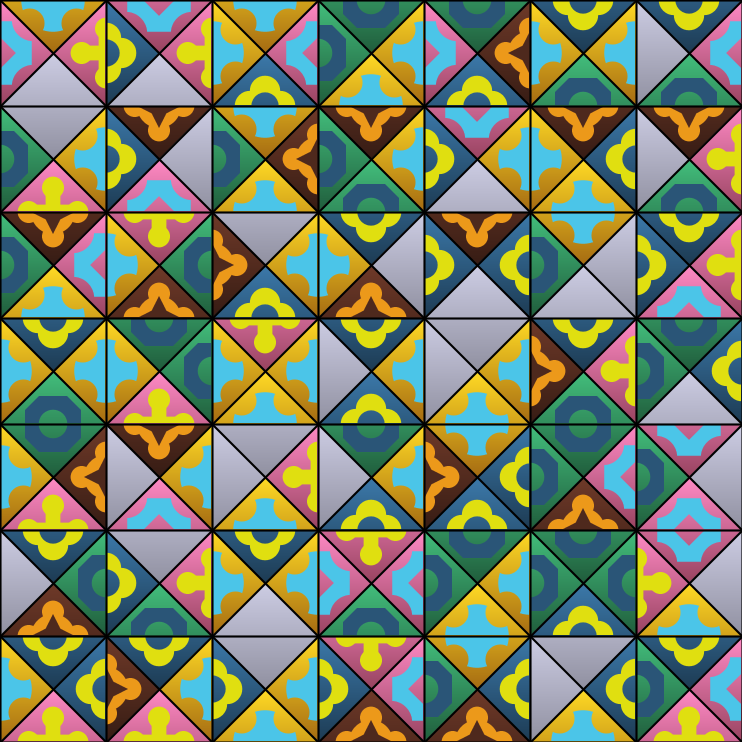
\includegraphics[width=35mm]{images/shuffled.png}
	\caption{Simplified puzzle with 7 by 7 tiles, with 6 colors}
	\label{fig:shuffled_example}
\end{figure}

\begin{figure}[h]
	\centering
	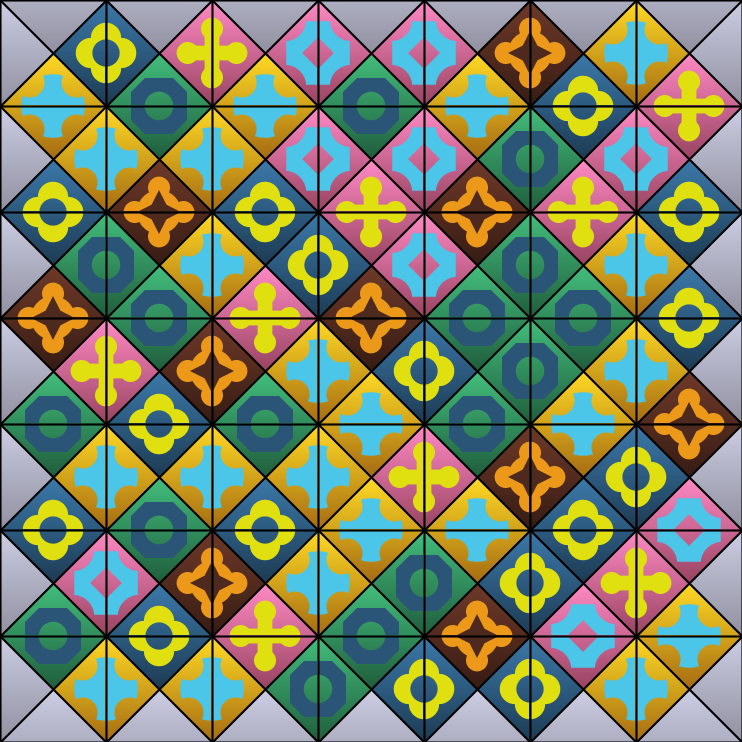
\includegraphics[width=35mm]{images/solved.png}
	\caption{Solution to the above puzzle}
	\label{fig:solved_example}
\end{figure}

Each piece has its edges marked with different shape and colour combinations, henceforth called colors. Each must precisely match the neighboring piece's edge when the puzzle is solved. Since the pieces are symmetrical, each can be placed in four different positions achieved by rotating the piece. Pieces that will sit on a corner or borderline tile can be easily distinguished from all the other, as they have a gray edge. There are 22 colors, not counting these gray edges.


\subsection{Normal approaches to solving the problem}\label{sec:normal_approaches}

We have found that the most common approaches that solve these kinds of problems can fall into one of two types: swap and iterative. Swap solutions always start with a complete board, and then use the rotate and swap operations in order to improve the board's state. Iterative approaches place pieces progressively, according to a certain criteria and can backtrack to any previous state if they determine that no good solution will be found from that point onward.

\subsubsection{The swap approach}\label{sec:swap_approach}

As said before, swap approaches begin by placing all the available pieces in the board, then use the swap and rotate operations to improve the board's state. There are plenty algorithms that can achieve this, like hill-climbing, tabu search and simulated annealing. These approaches evaluate the board's state and try to find which sequence of operations will achieve the greatest score possible (which in turn will mean a solved puzzle).

Evidently, the starting position of the pieces in the puzzle will also play an important part on the rest of the solving process. (Explain why?)

\subsubsection{The iterative approach}\label{sec:iterative_approach}

Iterative solutions try to place the pieces progressively, usually following some kind of pattern.
(Describe here most common patterns that can be used.)

\section{Genetic Algorithms}\label{sec:genetic_algorithms}

(Methodologies and approaches taken when trying new methods to improve solving times of simplified Eternity II puzzles)

Genetic algorithms (GA) are search algorithms that work by combining two (or more) \textit{parent} states in order to maximize the amount of information passed on to the next search step, instead of modifying a single state. These kind of algorithms have been proven useful in solving many kinds of problems, including board games problems, such as the \textit{n queens} problem\cite{eastridge}.

\subsection{Methodology}\label{sec:methodology}

% FIXME: tá péssimo
\subsubsection{Chromosome} The chromosome to be used in both the evaluation by the fitness function and the breeding methods is the board itself

\subsubsection{Fitness function}\label{sec:fitness-function}

The fitness function used to evaluate the quality of the boards is given by:

\begin{figure}[h]
	\begin{equation}
		fitness = \frac{n\_matching\_edges}{total\_matching\_edges}
	\end{equation}
	\caption{Fitness function for evaluating boards}
	\label{fig:eq:fitness_function}
\end{figure}

where \textit{n\_matching\_edges} represents the number of matching edges between all pieces of the board for the current state, and \textit{total\_matching\_edges} the number of matching edges for an $n*n$ board. As such, \textit{fitness} will yield a value between $[0.0, 1.0]$, with higher values corresponding to fitter boards. A fitness of $1.0$ means a board is correctly solved.

\subsubsection{Breeding}\label{sec:breeding}

Starting out with \textit{n} random permutations of the same board, the fittest half of the population is selected for breeding, using an ?elitist? selection approach. These specimens are then bred and their genetic code is crossed-over according to very specific rules:

\begin{itemize}
	\item If both parents have compatible features, use both features on both descendants in order to create fitter boards
	\item If both parents have incompatible features, select the highest scoring feature from each parent and use it as a starting point for each of the descendants
	\item The rest of the genetic code (pieces) not originated from the feature selection is then placed on the descendant boards using a simple (no backtracking) linear constructive method
	\item Mutations are then performed on a random set of pieces by rotating them in order to try and improve the overall fitness of the board
\end{itemize}

\subsection{Implementation}\label{sec:implementation}

\subsubsection{Feature Extraction}\label{sec:feature_extraction}

\subsubsection{Eternity II Editor}\label{sec:eternity2_editor}

(Why are we using Eternity II Editor and how we linked the previously developed solution with it)

\section{Results}\label{sec:results}

(Experimental results obtained from the application of the new methodologies to the diamonds board approach)

\section{Conclusions}\label{sec:conclusions}

(Conclusions go here)
%
% ---- Bibliography ----
%
\bibliographystyle{plain}
\bibliography{mpes}
\end{document}

